\documentclass[../Main.tex]{subfiles}

\begin{document}
\chapter{Teoremas de conservación}

\intro{
    Voy a tomar como inicio el mismo que menciono mi JTP, Pablo Gaztañaga,
cuando empezo esta segunda parte. Si uno le tendria que resumir a un amigo
que rindio en la primera parte, osea el primer parcia. Que le dirias? Cuando
lo dijo hubo un silencio y es obvio si por clase eramos unos 20, con toda la
furia, de los cuales casi menos de la mitad habiamos aprobado el primer
parcial. Pero la respuesta que Pablo queria se menciono en una voz al fondo
del aula. En esta segunda se basa en lo mismo que la primera y es la ecuacion
de Newton. En muchos libros este tema se lo menciona como las primera
integrales de la ecuacion de Newton.
}

\begin{minipage}[t]{0.3\textwidth}
\begin{figure}[H]
    \centering
    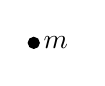
\begin{tikzpicture}

        % Esto representa una particula
        \filldraw[black] (0,0) circle (2pt) node[anchor=west]{$m$};

    \end{tikzpicture}
    \caption{Una particula libre que tiene masa y velocidad.}
    \label{fg:unaparticula}
\end{figure}

\end{minipage}
\hfill
\begin{minipage}[t]{0.6\textwidth}

\section{Impulsó lineal}

Supongamos que nosotros querremos describir una particula como en la 
figura (). Si, es solo una particula que pareciera ser que no se ve afectada
por nada. Si nosotros aplicamos lo que vimos en la primera parte de la materia
tendriamos que la ecuacion de Newton para la particual es la siguiente

\begin{equation}
    m \cdot \vec{a} = \sum \vec{F} \ .
\label{eq:sumP}
\end{equation}

Pero ahora vamos hacer un truco, que en realidad se hace en la primera parte de 
la materia, y es mirar a la aceleración como la deriva de la velocidad respecto
del tiempo

\begin{equation}
    \vec{a} = \frac{\partial \vec{v}}{\partial t} \ .
\end{equation}

Con esto podemos reemplazar en la ecuacion \ref{eq:sumP}. Ademas, una propiedad
de cuando uno deriva es que puede sacar las constantes que esten multiplicando
a la variable que estemos derivando y como para este caso la masa es una
constante voy hacer lo siguiente y es el paso inverso, meter la masa adentro de
la derivada.

\begin{equation}
    m \cdot \frac{\partial \vec{v}}{\partial t} = \sum \vec{F}
\end{equation}
\begin{equation*}
    \Downarrow
\end{equation*}
\begin{equation*}
    \frac{\partial}{\partial t} \left( m \cdot \vec{v} \right) = \sum \vec{F} \ .
\end{equation*}

La expresión que se encuentra dentro de los paréntesis es lo que en fisica se 
denomina como impulso lineal

\begin{equation}
    \vec{P} = m \cdot \vec{v}
\label{eq:impLineal}
\end{equation}
como la velocidad $\vec{v}$ es un vector, el impulso lineal $\vec{P}$ es
propiamente un vector.

Este mismo analisis del impulso lineal no se limita al caso de una particula,
sino que se puede realizar para un sistemas de $N$ partículas que interactuan
entre si.
Veamos el caso que se muestra en la figura (), podemos ver un sistema de 3
particulas que interactuan entre si de tal modo que ninguna de ellas mueve a la 
otra. El primer paso es poner las ecuaciones de Newton para cada una de las
particulas.

Para la particula 1 tenemos
\begin{equation*}
    m_1 \cdot \vec{a} _1 = \vec{F} _{12} + \vec{F} _{13} \ .
\end{equation*}

\end{minipage}
\newpage
\begin{minipage}[t]{0.3\textwidth}
\end{minipage}
\hfill
\begin{minipage}[t]{0.6\textwidth}

Para la particula 2 tenemos
\begin{equation*}
    m_2 \cdot \vec{a} _2 = \vec{F} _{21} + \vec{F} _{23} \ .
\end{equation*}

Para la particula 3 tenemos
\begin{equation*}
    m_3 \cdot \vec{a} _3 = \vec{F} _{31} + \vec{F} _{32} \ .
\end{equation*}

Ahora podriamos sumar las ecuaciones de Newton de todas las particulas,
obteniendo

\begin{equation*}
     m_1 \cdot \vec{a} _1 + m_2 \cdot \vec{a} _2 + m_3 \cdot \vec{a} _3 = \vec{F} _{12} + \vec{F} _{13} + \vec{F} _{21} + \vec{F} _{23} + \vec{F} _{31} + \vec{F} _{32} \ .
\end{equation*}

Antes de hacer el truco de ver que la aceleracion es la derivada de la
velocidad respecto del tiempo, me gustaria hacer un comentario sobre las
fuerzas. Mas que nada me intera los pares, por ejemplo la fuerza $\vec{F} _{12}$
y $\vec{F} _{21} $. Se puede ver que ambas tiene direcciones opuestas por la
figura () pero ademas sabemos que estas son de igual modulo porque es una
fuerza de interaccion, por lo que la suma entre $\vec{F} _{12}$ y $\vec{F} _{21}$.
da cero. Y esto mismo podriamos hacer para cada par de fuerza interna asi que
voy a reescribir la ecuacion anterior con los pares entre parentesis.

\begin{equation*}
     m_1 \cdot \frac{\partial \vec{v} _1}{\partial t} + m_2 \cdot \frac{\partial \vec{v} _2}{\partial t} + m_3 \cdot \frac{\partial \vec{v} _3}{\partial t} = (\vec{F} _{12} + \vec{F} _{21}) + (\vec{F} _{23} + \vec{F} _{32}) + (\vec{F} _{13} + \vec{F} _{31})
\end{equation*}
\begin{equation*}
    \Downarrow
\end{equation*}
\begin{equation*}
   \frac{\partial}{\partial t} \left(m_1 \cdot \vec{v} _1 + m_2 \cdot \vec{v} _2 + m_3 \cdot \vec{v} _3 \right) =  0 + 0 + 0
\end{equation*}
\begin{equation*}
    \Downarrow
\end{equation*}
\begin{equation}
    \frac{\partial}{\partial t} \left(\vec{P} _1 + \vec{P} _2 + \vec{P} _3 \right) = \frac{\partial \vec{P}}{\partial t} = 0 \ .
\end{equation}

De esta ultima expresion tenemos mucho para hablar. Lo primero es que la suma
de cada $\vec{P} _i$ donde $i$ es la cantidad de particulas en el sistema que
estemos analizando, nos da como resultado el $\vec{P}$ del sistema. Lo segundo
que nos dice la expresion es que derivada del impulso lineal del sistema
respecto del tiempo del tiempo es cero. Esto nos indica que para todo $t$ el 
impulso lineal es constante. En otras palabras, que el impulso lineal se
conserva para todo $t$.

\begin{equation}
    \vec{P} = \vec{P} _1 + \vec{P} _2 + \vec{P} _3 = m_1 \cdot \vec{v} _1 + m_2 \cdot \vec{v} _2 + m_3 \cdot \vec{v} _3 = cte \ .
    \label{eq:sistP}
\end{equation}

\end{minipage}
\newpage
\begin{minipage}[t]{0.3\textwidth}
\end{minipage}
\hfill
\begin{minipage}[t]{0.6\textwidth}

Ahora podrimos pensar el mismo ejemplo de las 3 particulas pero ahora teniendo
en cuenta que tienen una fuerza externa, por ejemplo que todas esten cayendo
por lo que se ven afectadas por su peso. Para el caso de las fuerzas internas
seguiria valiendo lo mismo solo que ahora si miramos el sistema de las 3
particulas vemos que la fuerza peso de cada una no se cancela.

\begin{equation*}
    \frac{\partial}{\partial t} \left(\vec{P} _1 + \vec{P} _2 + \vec{P} _3 \right) = \frac{\partial \vec{P}}{\partial t} = m_1 \cdot \vec{g} + m_2 \cdot \vec{g} + m_3 \cdot \vec{g}
\end{equation*}
como podemos ver ahora el impulso lineal no se conserva. Eso quiere decir que
si calculamos el $\vec{P}$ para un $t_0$ no va a ser igual a un $\vec{P}$ para
un $t$ futuro o posterior. Pero lo que si podemos calcular es la diferencia
del impulso lineal.

\begin{equation*}
    \frac{\partial \vec{P}}{\partial t} = m_1 \cdot \vec{g} + m_2 \cdot \vec{g} + m_3 \cdot \vec{g}
\end{equation*}
\begin{equation*}
    \Downarrow
\end{equation*}
\begin{equation*}
    \partial \vec{P} = ( m_1 \cdot \vec{g} + m_2 \cdot \vec{g} + m_3 \cdot \vec{g} ) \cdot \partial t
\end{equation*}
\begin{equation*}
    \Downarrow
\end{equation*}
\begin{equation*}
    \int _{\vec{P_I}}^{\vec{P_F}} \partial \vec{P} = \int _{t_I}^{t_F} m_1 \cdot \vec{g} \cdot \partial t + \int _{t_I}^{t_F} m_2 \cdot \vec{g} \cdot \partial t +\int _{t_I}^{t_F} m_3 \cdot \vec{g} \cdot \partial t
\end{equation*}
\begin{equation*}
    \Downarrow
\end{equation*}
\begin{equation*}
    \vec{P_F} - \vec{P_I} = \Delta \vec{P} = m_1 \cdot \vec{g} \cdot (t_F - t_I) + m_2 \cdot \vec{g} \cdot (t_F - t_I) + m_3 \cdot \vec{g} \cdot (t_F - t_I)
\end{equation*}
Una mencion de este caso y es que uno podria agarrar un interavalo de tiempo
tan chico para que todos los terminos que estan a la derecha tiendan a cero. Y
si lo pongo asi podria decir que el impulso lineal se conserva pero esto solo 
me serviria si quiero buscar la velocidad en un instante muy corto de tiempo.

En resumen, el impulso lineal se puede calcular de la siguiente manera

\begin{equation*}
    \vec{P} = \sum _i m_i \cdot \vec{v} _i
\end{equation*}
\begin{equation*}
    \frac{\partial \vec{P}}{\partial t} = \sum \vec{F}^{EXT}
\end{equation*}

\end{minipage}
\newpage
\begin{minipage}[t]{0.3\textwidth}
\end{minipage}
\hfill
\begin{minipage}[t]{0.6\textwidth}

\section{Centro de masa y Velocidad centro de masa}

Voy a seguir con el ejemplo del sistema de 3 masas de la figura () y voy a
partir de la ecuacion \ref{eq:sistP} para seguir desarrollando un poco mas.

El paso siguiente pensar la velocidad como la derivada de la posicion respecto
del tiempo. Por lo que obtenes que 

\begin{equation*}
    \vec{P} = m_1 \cdot \frac{\partial \vec{r} _1}{\partial t} + m_2 \cdot \frac{\partial \vec{r} _2}{\partial t} + m_3 \cdot \frac{\partial \vec{r} _3}{\partial t}
\end{equation*}
\begin{equation*}
    \Downarrow
\end{equation*}
\begin{equation*}
    \vec{P} = \frac{\partial}{\partial t}(m_1 \cdot \vec{r} _1 + m_2 \cdot \vec{r} _2 + m_3 \cdot \vec{r} _3)
\end{equation*}
ahora si a esta expresion la dividimos por la suma de todas las masas obtenemos
\begin{equation}
    \frac{\vec{P}}{m_1 + m_2 + m_3} = \frac{\partial}{\partial t} \left(\frac{m_1 \cdot \vec{r} _1 + m_2 \cdot \vec{r} _2 + m_3 \cdot \vec{r} _3}{m_1 + m_2 + m_3} \right) = cte
    \label{eq:preRC}
\end{equation}

De esta ecuacion nos interesa lo que parece en el parentesis. Es lo que se
denomina como "Centro de Masa". 

\begin{equation}
    \vec{r} _{CM} = \frac{m_1 \cdot \vec{r} _1 + m_2 \cdot \vec{r} _2 + m_3 \cdot \vec{r} _3}{m_1 + m_2 + m_3}
    \label{eq:rc}
\end{equation}

Este es un vector que apunta a un punto imaginario que mejor representa al
sistema de masas que estemos analizando. Digo imaginario porque no es
necesario que este punto que mejor representa al sistema este en una de las
masas. Existe el caso que eso pase y es cuando una de las es muchisimo mayor
a las otras. Por ejemplo, si $m_1$ tiende a infinito, el centro de masa
va a estar en la misma posicion que la particula 1.

Ahora me gustaria hablar sobre la derivada del centro de masa y es la velocidad
centro de masa. Al igual que en la primera parte de cinematica, el vector
posicion al derivarlo respecto del tiempo se obtiene la velocidad.

\begin{equation*}
    \frac{\vec{P}}{m_1 + m_2 + m_3} = \vec{v}_{CM} = \frac{\partial}{\partial t} \left(\vec{r} _{CM}\right) = cte
\end{equation*}
\begin{equation*}
    \Downarrow
\end{equation*}
\begin{equation}
    \vec{v}_{CM} = \frac{m_1 \cdot \vec{v} _1 + m_2 \cdot \vec{v} _2 + m_3 \cdot \vec{v} _3}{m_1 + m_2 + m_3}
    \label{eq:vc}
\end{equation}

\end{minipage}
\newpage
\begin{minipage}[t]{0.3\textwidth}
\end{minipage}
\hfill
\begin{minipage}[t]{0.6\textwidth}

En el caso donde la sumatoria de fuerzas externas de nuestro sistema sea cero.
Podremos ver que el Centro de masa se mueve como un MRU. Esto se puede ver
claro con el ejemplo de las 3 particulas porque al llegar a la expresión de
la velocidad centro de masa mediante podemos ver que esta igualado al impulso
lineal divido la suma de las masas, el impulso lineal era constante para todo
tiempo, las masas tambien lo son, entonces por tautologia la velocidad centro
de masa es constante. En general esto pasa para todo sistema donde la suma
de las fuerzas externas sea igual a cero.

Una expresion mas en general del centro de masa y la velocidad centro de masa
es la siguiente

\begin{equation*}
    \vec{r} _{CM} = \frac{\sum _i m_i \cdot \vec{r} _i}{\sum _i m_i}
\end{equation*}

\begin{equation*}
    \vec{v} _{CM} = \frac{\sum _i m_i \cdot \vec{v} _i}{\sum _i m_i}
\end{equation*}
\end{minipage}

\end{document}
